\documentclass[a4paper,11pt]{article}
\usepackage{graphicx}
\title{Software Requirements Specification \\ Bin-packing VM Consolidation Algorithm}
\author{Atchutuni Bhavana \\ Terli Venkatesh \\ Surineni Sampath Kumar}
\date{\today}

\begin{document}
	\maketitle
	 \pagebreak 
	 \tableofcontents
	 \pagebreak 

	\section{INTRODUCTION}
		\subsection{Product overview}
		This project takes as  input 
		\begin{itemize}
		  \item Physical machines and their capacities
		  \item Virtual machines and their capacity requirements
		  
		\end{itemize} 
		It computes the residual capacity in each physical machine after adding the 
		virtual machines. The physical machines are sorted in ascending order of their residual capacity. 
		The project provides the feature of consolidating the virtual machines in different physical machines into 
		minimum number of physical machines. Other features provided by this project are to switch off a physical machine by migrating the virtual machines in that physical machine into 
		others and switch on a physical machine. This project uses greedy bin packing algorithm. 
		\section{SPECIFIC REQUIREMENTS}
		\subsection{External Interface Requirements}
			\subsubsection{User Interfaces}
			
 			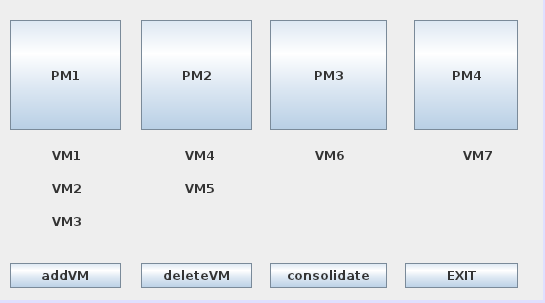
\includegraphics[height=8cm]{images/gui}
 			\\
 			\\
			The GUI displays 			
			\begin{itemize}
				\item All the physical machines
				\item Virtual Machines in each physical machine
				\item Buttons for adding a vm, deleting a vm, consolidation and to exit 
			\end{itemize}

			\subsubsection{Hardware Interfaces}
			No specific hardware module is being used for this project
			\subsubsection{Software Interfaces}
			No specific software module is being used for this project 
			\subsubsection{Communication Protocols}
			This project doesn’t use any communication protocols
		\subsection{Software Product Features}
			\begin{enumerate}
				\item {\bf Provides the ability to add a vm} \\
 				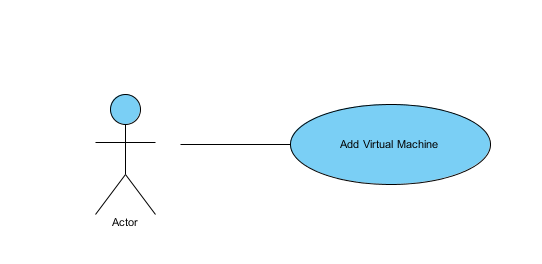
\includegraphics{images/usecase}
				\\This action is triggered by user clicking {\bf Add VM } Button. A new window appears with fields for  
				\begin{itemize}
				 \item VM ID
				 \item VM capacity
				\end{itemize}
				
				This would return \\
				{\bf On Success: }\\
				The GUI will be updated showing that new  VM that is added to existing PM.
				The residual capacity of the PM is calculated and updated to reflect in GUI\\\\
				{\bf On Failure: } \\
				{\bf Reason: No enough residual capacity to accomodate a VM}\\
				The user will get an error message that there is no enough space to add the given VM\\
				
				\item {\bf Provides the ability to delete a vm}\\
				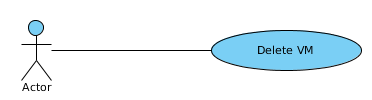
\includegraphics{images/delete}
				\\This action is triggered by user clicking {\bf Delete VM } Button. 
				\begin{itemize}
				 \item A new window appears with a drop down list of all the VM\textunderscore ID  that are 
				 present in the system.
				\end{itemize}
				
				This would return \\
				{\bf On Success: }\\
				The GUI will be updated showing that VM  is deleted from the PM.
				The residual capacity of the PM is calculated and update to reflect in GUI\\\\
				
				\item {\bf Ability to switch off a physical machine}\\
				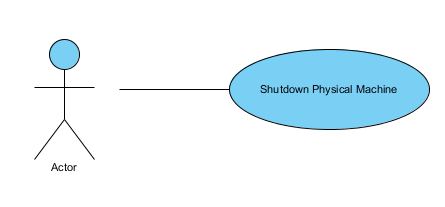
\includegraphics{images/shut}
				\\This action is triggered by user clicking on the PM which he wants to switch off. 
								
				This would result in \\\\
				{\bf On Success: }\\
				The software moves all the VM's into other PM's with sufficient residual capacity. Then the physical machine is shutdown.
			
				The GUI will be updated and the color of specified PM is changed showing that the selected PM is switched off.
				\\\\
				{\bf On Failure: } \\
				{\bf Reason: VM's in the selected PM cannot be accomodated in other PM's}\\
				The user will get a message stating that the VM's in the selected PM cannot be accomodated in other PM's.
				
				\item {\bf Ability to switch on a physical machine}\\
				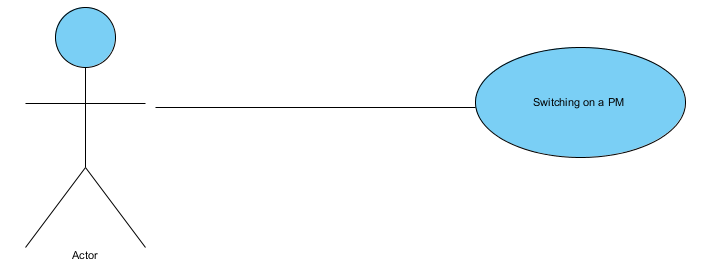
\includegraphics[scale=0.7]{images/onpm}
				\\This action is triggered by user clicking on the PM which he wants to switch on. 
				
				This would result in \\\\
				{\bf On Success: }\\
				The PM will be switched on. The color of the PM is changed from red to green to reflect the on 
				status of PM in GUI 
				
				
				
				\item {\bf Provides the ability to consolidate all VM's in minimum number of PM's}\\
				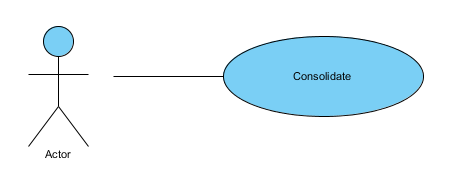
\includegraphics{images/consolidate}
 				\\This action is fired by user clicking the {\bf consolidate} Button. 
								
				This would result in \\\\
				{\bf On Success: }\\
				The software runs Bin packing algorithm. Moves the VMs into as few PMs as possible. Updates the GUI
				\\
				
				
				\item {\bf Ability to exit the program}\\
				\\This action is triggered by user clicking on the \textbf{Exit} button. 
				
				This would result in \\\\
				{\bf On Success: }\\
				All the resources are released and the system is exited.
				
				
				
				

			\end{enumerate}


\end{document}
